\documentclass{beamer}\usepackage[]{graphicx}\usepackage[]{color}
%% maxwidth is the original width if it is less than linewidth
%% otherwise use linewidth (to make sure the graphics do not exceed the margin)
\makeatletter
\def\maxwidth{ %
  \ifdim\Gin@nat@width>\linewidth
    \linewidth
  \else
    \Gin@nat@width
  \fi
}
\makeatother

\definecolor{fgcolor}{rgb}{0.345, 0.345, 0.345}
\newcommand{\hlnum}[1]{\textcolor[rgb]{0.686,0.059,0.569}{#1}}%
\newcommand{\hlstr}[1]{\textcolor[rgb]{0.192,0.494,0.8}{#1}}%
\newcommand{\hlcom}[1]{\textcolor[rgb]{0.678,0.584,0.686}{\textit{#1}}}%
\newcommand{\hlopt}[1]{\textcolor[rgb]{0,0,0}{#1}}%
\newcommand{\hlstd}[1]{\textcolor[rgb]{0.345,0.345,0.345}{#1}}%
\newcommand{\hlkwa}[1]{\textcolor[rgb]{0.161,0.373,0.58}{\textbf{#1}}}%
\newcommand{\hlkwb}[1]{\textcolor[rgb]{0.69,0.353,0.396}{#1}}%
\newcommand{\hlkwc}[1]{\textcolor[rgb]{0.333,0.667,0.333}{#1}}%
\newcommand{\hlkwd}[1]{\textcolor[rgb]{0.737,0.353,0.396}{\textbf{#1}}}%
\let\hlipl\hlkwb

\usepackage{framed}
\makeatletter
\newenvironment{kframe}{%
 \def\at@end@of@kframe{}%
 \ifinner\ifhmode%
  \def\at@end@of@kframe{\end{minipage}}%
  \begin{minipage}{\columnwidth}%
 \fi\fi%
 \def\FrameCommand##1{\hskip\@totalleftmargin \hskip-\fboxsep
 \colorbox{shadecolor}{##1}\hskip-\fboxsep
     % There is no \\@totalrightmargin, so:
     \hskip-\linewidth \hskip-\@totalleftmargin \hskip\columnwidth}%
 \MakeFramed {\advance\hsize-\width
   \@totalleftmargin\z@ \linewidth\hsize
   \@setminipage}}%
 {\par\unskip\endMakeFramed%
 \at@end@of@kframe}
\makeatother

\definecolor{shadecolor}{rgb}{.97, .97, .97}
\definecolor{messagecolor}{rgb}{0, 0, 0}
\definecolor{warningcolor}{rgb}{1, 0, 1}
\definecolor{errorcolor}{rgb}{1, 0, 0}
\newenvironment{knitrout}{}{} % an empty environment to be redefined in TeX

\usepackage{alltt}
\usetheme{Madrid}

%%%%% Packages %%%%%
\usepackage{algorithm}
\usepackage{csquotes}
\usepackage[round]{natbib}
\bibliographystyle{agsm}
\usepackage{algorithmic}
\usepackage{pgfpages}
\usepackage{ragged2e}
\usepackage{etoolbox}
\usepackage{lipsum}
\usepackage{subfig}
\apptocmd{\frame}{}{\justifying}{} 
\usepackage{xcolor}
\usepackage{dsfont}
\usepackage{tikz}
\usepackage{amsmath}
\usepackage{graphicx}
\usepackage{subfig}
\usepackage{mathtools}
\usepackage{xcolor}
\usepackage{comment}
\usepackage{appendixnumberbeamer}
%%%%% New Commands %%%%
\newcommand{\btheta}{\boldsymbol{\theta}}
\newcommand{\x}{\mathbf{x}}
\newcommand{\SUN}{\textrm{SUN}}
\newcommand{\X}{\mathbf{X}}
\newcommand{\T}{\textrm{T}}
\newcommand{\A}{\mathcal{A}}
\newcommand{\I}{\mathds{1}}
\newcommand{\hist}{\mathbb{H}_{t-1}}
\newcommand\myeq{\stackrel{\mathclap{\normalfont\mbox{def}}}{=}}
\def\app#1#2{%
  \mathrel{%
    \setbox0=\hbox{$#1\sim$}%
    \setbox2=\hbox{%
      \rlap{\hbox{$#1\propto$}}%
      \lower1.1\ht0\box0%
    }%
    \raise0.25\ht2\box2%
  }%
}
\def\approxprop{\mathpalette\app\relax}
%\pgfpagesuselayout{1 on 1}[a4paper,border shrink=5mm]
\title{}
\author[Wang, Zheng, Zito]{Carol Wang \and Xiaojun Zheng \and Alessandro Zito}
\institute[Stat 723]{Case Study 2 - Stat 723}
\date{\today}
\IfFileExists{upquote.sty}{\usepackage{upquote}}{}
\begin{document}

\begin{frame}
\titlepage
\end{frame}

\begin{frame}{Overview}
\tableofcontents
\end{frame}

%%%%%%%%%%%%%%%%%%%%%%%%%%%%%%%%%%%%%%%%%%%%%
%%%% Introduction                       
%%%%%%%%%%%%%%%%%%%%%%%%%%%%%%%%%%%%%%%%%%%%%
\section{Introduction}
\begin{frame}{Introduction}

\end{frame}

%%%%%%%%%%%%%%%%%%%%%%%%%%%%%%%%%%%%%%%%%%%%%
%%%% The Data                       
%%%%%%%%%%%%%%%%%%%%%%%%%%%%%%%%%%%%%%%%%%%%%
\section{Data}
\begin{frame}{Data}

\end{frame}
%%%%%%%%%%%%%%%%%%%%%%%%%%%%%%%%%%%%%%%%%%%%
\begin{frame}{Data}

\end{frame}

%%%%%%%%%%%%%%%%%%%%%%%%%%%%%%%%%%%%%%%%%%%%%
%%%% EDA                    
%%%%%%%%%%%%%%%%%%%%%%%%%%%%%%%%%%%%%%%%%%%%%
\begin{frame}{EDA (I) - Missing Data}
20\% missing in Last Review, and Reviews per month

\end{frame}

\begin{frame}{Data Cleaning}
- Remove the missing data, and use complete cases
- Use reviews per month as a measure for popularity
- Take log of price and popularity

\end{frame}

\begin{frame}{EDA (II) - Neighborhoods effects}

\begin{figure}
  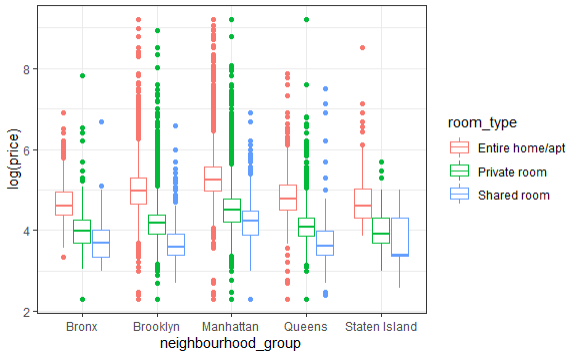
\includegraphics[width=\linewidth]{NG_eda.png}
\end{figure}
\end{frame}
\begin{frame}{EDA (II) - Neighborhoods effects}
\begin{figure}
  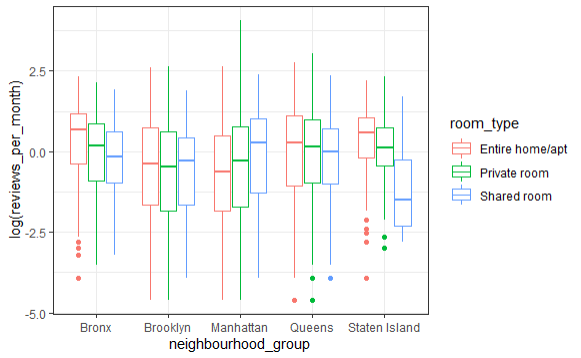
\includegraphics[width=\linewidth]{NG_eda_popu.png}
\end{figure}

\end{frame}

\begin{frame}{EDA (II) - Names effects}

\begin{figure}
  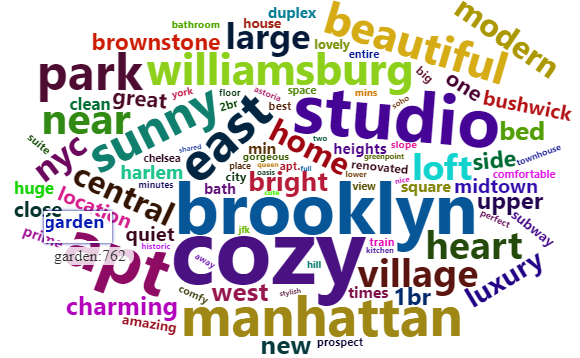
\includegraphics[width=\linewidth]{wordcloud.png}
\end{figure}

\end{frame}
%%%%%%%%%%%%%%%%%%%%%%%%%%%%%%%%%%%%%%%%%%%%%
%%%% Model 1                    
%%%%%%%%%%%%%%%%%%%%%%%%%%%%%%%%%%%%%%%%%%%%%
\section{Model (I) - ??}
\begin{frame}
Model assumptions are checked in the appendix.
\end{frame}

\section{Conclusions}
\begin{frame}{Conclusions}
\end{frame}

\begin{frame}
\frametitle{References}
\footnotesize{
\begin{thebibliography}{99} % Beamer does not support BibTeX so references must be inserted manually as below
	
	\bibitem[Li et al, 2013]{Li_Long_Duns} Li, D; Longnecker, M.P.; and Dunson, D.B. \\
	\newblock Lipid Adjustment for Chemical Exposures: Accounting for Concomitant Variables.\\
	\newblock \emph{Epidemiology}, Nov 2013

	
\end{thebibliography}
}
\end{frame}
%%%%%%%%%%%%%%%%%%%%%%%%%%%%%%%%%%%%%%%%%%%%%
%%%% Appendix                 
%%%%%%%%%%%%%%%%%%%%%%%%%%%%%%%%%%%%%%%%%%%%%
\appendix
\section{Appendix}







\end{document}
